\let\negmedspace\undefined
\let\negthickspace\undefined
\documentclass[journal,12pt,twocolumn]{IEEEtran}
\usepackage{gensymb}
\usepackage{amssymb}
\usepackage[cmex10]{amsmath}
\usepackage{amsthm}
\usepackage{float}
\usepackage[export]{adjustbox}
\usepackage{bm}
\usepackage{longtable}
\usepackage{enumitem}
\usepackage{mathtools}
 \usepackage{tikz}
\usepackage[breaklinks=true]{hyperref}
\usepackage{listings}
\usepackage{color}                                            %%
\usepackage{array}                                            %%
\usepackage{longtable}                                        %%
\usepackage{calc}                                             %%
\usepackage{multirow}                                         %%
\usepackage{hhline}                                           %%
\usepackage{ifthen}                                           %%
\usepackage{lscape}     
\usepackage{multicol}
% \usepackage{enumerate}
\DeclareMathOperator*{\Res}{Res}
\renewcommand\thesection{\arabic{section}}
\renewcommand\thesubsection{\thesection.\arabic{subsection}}
\renewcommand\thesubsubsection{\thesubsection.\arabic{subsubsection}}
\renewcommand\thesectiondis{\arabic{section}}
\renewcommand\thesubsectiondis{\thesectiondis.\arabic{subsection}}
\renewcommand\thesubsubsectiondis{\thesubsectiondis.\arabic{subsubsection}}
\hyphenation{op-tical net-works semi-conduc-tor}
\def\inputGnumericTable{}                                 %%
\lstset{
frame=single, 
breaklines=true,
columns=fullflexible
}
\begin{document}

\raggedbottom
\setlength{\parindent}{0pt}
\vspace{3cm}
\title{AI1110 - Assignment 2}
\author{Vedant Bhandare\\CS21BTECH11007}
\maketitle
\newpage
\bigskip
\renewcommand{\thefigure}{\theenumi}
\renewcommand{\thetable}{\theenumi}
\maketitle

Download all python codes from 
\begin{lstlisting}
https://github.com/TYCN129/AI1110-Assignments/tree/main/Assignment%202/Codes
\end{lstlisting}
%
and latex codes from 
%
\begin{lstlisting}
https://github.com/TYCN129/AI1110-Assignments/tree/main/Assignment%202
\end{lstlisting}
\textbf{ICSE class 12 - 2019 paper}

\section{\textbf{QUESTION - 18}}
Draw a sketch and find the area bounded by the curve $x^2 = y$ and $x + y = 2$
\section{\textbf{SOLUTION}}
Let us find out the points of intersection of the two curves. We have the curves
\begin{align}
    x^2 &= y\\
    x + y &= 2
\end{align}
Substituting $y = x^2$ (from equation 1) in equation 2.
\begin{align}
    x + x^2 &= 2\\
    x^2 + x - 2 &= 0\\
    (x + 2)(x - 1) &= 0\\
    \fbox{x = -2, 1}
\end{align}
Substituting value of $x$ in equation 2, we get.
\begin{align}
    \fbox{y = 4, 1}
\end{align}
Let $(x_1,y_1)$ and $(x_2,y_2)$ be the two points of intersection.
\begin{align}
    (x_1,y_1) &= (-2,4)\\
    (x_2,y_2) &= (1,1)
\end{align}
\begin{figure}[H]
    \centering
    \includegraphics[width=\columnwidth]{Figures/Question.png}
\end{figure}
\begin{center}
    Figure 1: Graph Plot
\end{center}
We need to find out the area of the shaded region shown below
\begin{figure}[H]
    \centering
    \includegraphics[width=\columnwidth]{Figures/Sketch.png}
\end{figure}
\begin{center}
    Figure 2: Region bound by the two curves
\end{center}
From the figure,
\begin{center}
Area between the curves(A)= Area of trapezium ABCD($A_1$) - Area under the curve $x^2 = y$($A_2$)
\end{center}

\clearpage

\subsection{\textbf{Area of trapezium ABCD (A_1)}}
\begin{figure}[H]
    \centering
    \includegraphics[width=\columnwidth]{Figures/trapezium.png}
\end{figure}
\begin{center}
    Figure 3: Trapezium ABCD
\end{center}
\begin{align}
    A_1 &= \frac{1}{2}\times(AB + CD)\times AD\\
    A_1 &= \frac{1}{2}\times(4 + 1)\times 3
\end{align}
\begin{center}
    \fbox{A_1 = 7.5 sq.units}
\end{center}
\subsection{\textbf{Area under the curve $x^2 = y$ (A_2)}}
\begin{figure}[H]
    \centering
    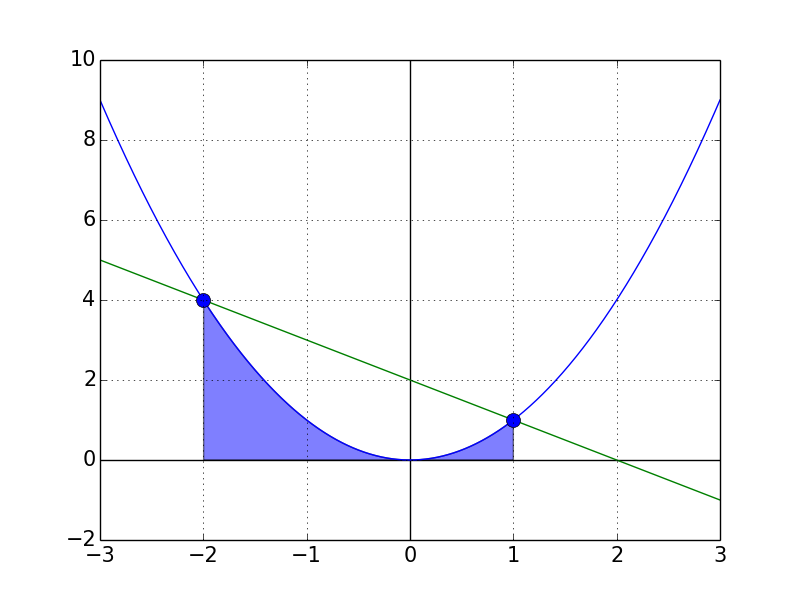
\includegraphics[width=\columnwidth]{Figures/x^2.png}
\end{figure}
\begin{center}
    Figure 4: Region below curve $x^2 = y$
\end{center}
\begin{align}
    A_2 &= \int_{-2}^{1} x^2 \, dx\\
    A_2 &= \frac{x^3}{3}\Biggr|_{-2}^{1}\\
    A_2 &= \frac{(1)^3}{3} - \frac{(-2)^3}{3}
\end{align}
\begin{center}
    \fbox{A_2 = 3 sq.units}
\end{center}    
Therefore,
\begin{align}
    A &= A_1 - A_2\\
    A &= 7.5 - 3\\
\end{align}
\begin{center}
    \textbf{\fbox{A = 4.5 sq.units}}
\end{center}
\begin{figure}[H]
    \centering
    \includegraphics[width=\columnwidth]{Figures/Sketch.png}
\end{figure}
\begin{center}
\textbf{The area bound by the curves $x^2 = y$ and $x + y = 2$ is 4.5 sq.units}
\end{center}
\end{document}